%*************************************************************
% Master Project                                             *
% Ing. Minerva Gabriela Vargas Gleason                       *
% IAI - Institute of Artificial Intelligence                 *
% Universität Bremen                                         *
%                                                            *
% pdfLaTex                                                   *
% Editor: TeXnicCenter                                       *
%*************************************************************

\chapter{Methodology}

This chapter describes ......

\section{Basics}


\section{System architecture (diagram)}
\section{Perception}
\subsection{Object Database}
YAML file, Markers
\subsection{Grasping Poses}
\subsection{RViz integration}

\section{Motion Controller}
\label{sec:motion_controller}

The motion control system used  to generate and control the movement of the robot is called Giskard (section \ref{subsec:giskard}). Giskard uses \textit{qpOASES}\footnote{\url{https://projects.coin-or.org/qpOASES}}  to calculate a trajectory for each joint. As stated by \citet{qpoases},  qpOASES is an open-source optimization software that can solve quadratic programming (QP) problems of the form:
\begin{equation}
\underset{x}{\min}\ c(x)\ =\  \underset{x}{\min}\ \left( \frac{1}{2} \ x' \ \textbf{H} \ x + x' \ g(\omega_{0}) \right)
\label{eq:cost_in}
\end{equation}
Where $H \in \Re^{nV\times nV}$ is a symmetric and positive (semi-)definite Hessian matrix and $g \in \Re^{nV}$ is a gradient vector that depends on the parameter $\omega_{0}$. The software tries to minimize the cost function $c(x)$. This minimization is subject to some constraints:
$$lb(\omega_{0})\ \leq\ x\ \leq\ ub(\omega_{0})$$
$$lbA(\omega_{0})\ \leq\ \textbf{A}x\ \leq\ ubA(\omega_{0})$$
where $lb$, $ub \in \Re^{nV}$ are the lower and upper constraint bound vectors of $x$, the matrix $A \in \Re^{nC\times nV}$ is the constrain matrix with the lower and upper constraint boundary vectors $lbA$, $ubA \in \Re^{nV}$. Equality constraints can be achieved by setting equal upper and lower boundaries.
 
Several simple controllers were built and tested in order to understand the characteristics of the trajectories obtained using qpOASES. The controllers describe a two degree of freedom (DOF) linear manipulator. A state vector, $\vec{s}\ \in\ \Re^{nV}$, that describes the system is used as the variable to minimize of the cost function:
\begin{equation}
 \vec{s} = [\dot{\ q_{0}} \ \ \dot{q_{1}} \ \ \epsilon ]^{T}
\end{equation}
where $\dot{q_{0}}$ is the velocity of the first joint, $\dot{q_{1}}$ the velocity of the second joint and $\epsilon$ is a slack variable. Introducing this vector in the cost function and setting the gradient $g$ to zero:
\begin{equation}
\underset{\vec{s}}{\min}\ c(\vec{s})\ =\  \underset{\vec{s}}{\min}\ \left( \frac{1}{2} \ \vec{s}' \ \textbf{H} \ \vec{s} \right)
\label{eq:cost}
\end{equation}
with the minimization constraints given by:
\begin{equation}
\vec{lb}(t)\ \leq\ \vec{s}\ \leq\ \vec{ub}(t)
\label{eq:constrain}
\end{equation}
\begin{equation}
\vec{lbA}(t)\ \leq\ \textbf{A} \vec{s}\ \leq\ \vec{ubA}(t)
\label{eq:constrainA}
\end{equation}
We define different weights for each parameter of the state vector $\vec{s}$ by setting the $H$ matrix to:
\begin{equation*}
\textbf{H}\ =\ diag(\vec{\omega})
\end{equation*}
with the weight vector $\vec{\omega} \in \Re^{nV}$. These weights allows us to prioritize the movement of one specific joint over the others, considering that the cost function for the 2 DOF controller from eq \ref{eq:cost} is given by:
\begin{equation}
c(\vec{s})\ =\ \frac{1}{2} \ \vec{s}' \ \textbf{H} \ \vec{s} =\ \frac{1}{2} \ (\ \dot{q_{0}}^{2}\omega_{1} + \dot{q_{1}}^{2}\omega_{2} + \epsilon^{2}\omega_{3})
\end{equation}

The software will try to minimize the cost of solving the problem by setting a higher value for the variables with a lower weight.

The result of this minimization problem is the velocity required by each joint to reach a goal position in a certain time. This can be set as an equality constraint:
\begin{equation}
error\ =\ q_{eef,des} - q_{eef}
\label{eq:init_error}
\end{equation}
\begin{equation}
error\ \ \leq\ \ \dot{\ q_{0}} + \dot{\ q_{1}} + \epsilon\ \ \leq\ \ error
\label{eq:goal}
\end{equation}
where $q_{eef,des}$ is the desired position of the end effector (EEF) and $q_{eef}$ the current position of the EEF. The position error can be used as a velocity goal if we suppose that we want to cover the distance error un one time unit. Velocity constraints are also established for each joint:
\begin{equation}
-\dot{q}_{0,max}\ \ \leq\ \ \dot{\ q_{0}}\ \leq\ \ \dot{q}_{0,max}
\end{equation}
\begin{equation}
-\dot{q}_{1,max}\ \ \leq\ \ \dot{\ q_{1}}\ \leq\ \ \dot{q}_{1,max}
\end{equation}
The software will try to find the velocity required by each joint to minimize the position error in one time step. Since the joints have velocity limits, it might not be possible to set velocities that satisfy the constraint set by eq \ref{eq:goal}, that is why the slack variable $\epsilon$ was introduced, with the constraints: 
\begin{equation}
-\epsilon{max}\ \ \leq\ \ \epsilon\ \leq\ \ \epsilon{max}
\end{equation}
where $\epsilon{max}\ \gg\ q_{0,max},\ q_{1,max}$. The weight of the slack value is higher than the ones of the joint velocities, so the software will try to give a higher value to the velocities than to the slack variable.

The joint limits also have to be taken into consideration:
\begin{equation}
-q_{0,max} - q_{0}\ \ \leq\ \ \dot{\ q_{0}}\ \leq\ \ q_{0,max} - q_{0}
\end{equation}
\begin{equation}
-q_{1,max} - q_{1}\ \ \leq\ \ \dot{\ q_{1}}\ \leq\ \ q_{1,max} - q_{1}
\end{equation}
These constraints will reduce the joint velocities when they are approaching the limits until they reach zero at joint limit. The obtained velocity is the velocity the joints would have to instantaneously reach to get to the goal potion in one time instant. However, due to physical limitations, joints can not immediately reach maximum velocity on one time step, so acceleration limits have to be established:
\begin{equation}
-a_{0,max}\ \ \leq\ \ \dot{\ q_{0}}\ \leq\ \ a_{0,max}
\label{eq:accel0}]
\end{equation}
\begin{equation}
-a_{1,max}\ \ \leq\ \ \dot{\ q_{1}}\ \leq\ \ a_{1,max}
\label{eq:accel1}
\end{equation}
Combining equations \ref{eq:goal} to \ref{eq:accel1} to create the constraint bound vectors from equations \ref{eq:constrain} and \ref{eq:constrainA}, we obtain:
\begin{equation}
\left( \begin{array}{c}
-\dot{q}_{0,max} \\
-\dot{q}_{1,max} \\
-\epsilon_{max} \\
\end{array}
\right)	\leq 
\left[ \begin{array}{cccc}
\omega_{1} & 0 & 0 \\
0 & \omega_{2} & 0 \\
0 & 0 & \omega_{3} \\
\end{array}
\right] *
\left( \begin{array}{c}
\dot{q}_{0} \\
\dot{q}_{1} \\
\epsilon \\
\end{array}
\right) 
\leq \left( \begin{array}{c}
\dot{q}_{0,max} \\
\dot{q}_{1,max} \\
\epsilon_{max} \\
\end{array}
\right)
\label{eq:state_constr}
\end{equation}
$\ $ \\
\begin{equation}
\left( \begin{array}{c}
error \\
-q_{0,max} - q_{0} \\
-q_{1,max} - q_{1} \\
a_{0,min\_lim} \\
a_{1,min\_lim} \\
\end{array}
\right)	\leq 
\left[ \begin{array}{cccc}
1 & 1 & 1 \\
1 & 0 & 0 \\
0 & 1 & 0 \\
1 & 0 & 0 \\
0 & 1 & 0 \\
\end{array}
\right] *
\left( \begin{array}{c}
\dot{q}_{0} \\
\dot{q}_{1} \\
\epsilon \\
\end{array}
\right) 
\leq \left( \begin{array}{c}
error \\
q_{0,max} - q_{0} \\
q_{1,max} - q_{1} \\
a_{0,max\_lim} \\
a_{1,max\_lim} \\
\end{array}
\right)
\label{eq:a_constr}
\end{equation}

The constrains set by these equations are the groundwork for the basic controllers explained in the following subsections. All these cases simulate a translational 2 DOF system, the goal is to position the EEF at a given distance (goal). The initial position of each joint is given, as well as a goal for the EEF. The initial velocity of the joints is assumed to be zero, but other initial conditions could also be set.

\subsection{Simple 2 DOF controller}
A proportional gain for the joints goal is introduced in order to reduce the number of iterations the program required to solve the problems. In other words, the proportional gain can be used to increase the joint velocities. Rewriting equation \ref{eq:init_error}:
\begin{equation}
error\ =\ p\ *\ \left(q_{eef,des} - q_{eef}\right)
\end{equation}


Figures \ref{fig:basic_eef} and \ref{fig:basic} show the position and velocity of a 2 DOF manipulator, whose trajectory is calculated using equations \ref{eq:state_constr} and \ref{eq:a_constr} to obtain the joint velocity in each time step. Figure \ref{fig:basic_eef}  shows the EEF position (blue), velocity (orange) and the goal position (green), while figure \ref{fig:basic} shows the position and velocity of the joints $q_{0}$ and $q_{1}$.

\begin{figure}[H]
	\centering
	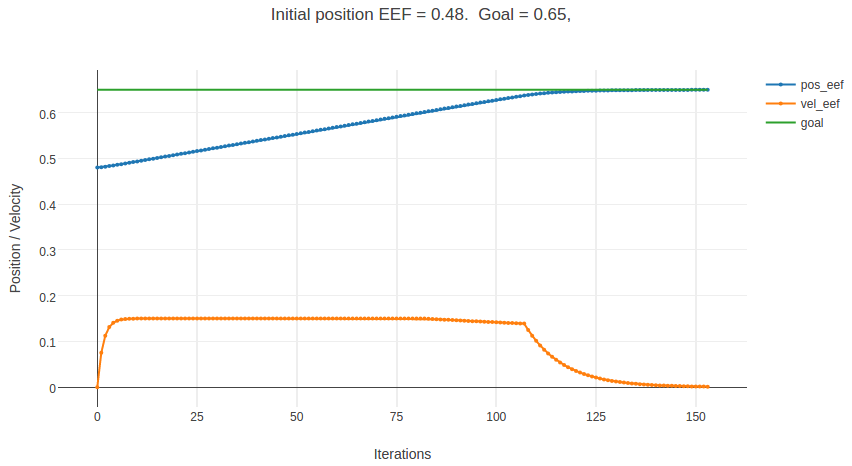
\includegraphics[width=0.9\linewidth, angle=0]{controllers/basic_eef.png}
	\vspace{-10pt}
	\caption[Basic 2 DOF controller: EEF trajectory.] {EEF trajectory. Initial acceleration is limited by constraints. Velocity decreases as EEF aproaches the goal position.}
	\vspace{-15pt}
	\label{fig:basic_eef}
\end{figure}
\begin{figure}[H]
	\centering
	\begin{subfigure}[][Joint $q_{0}$]
		{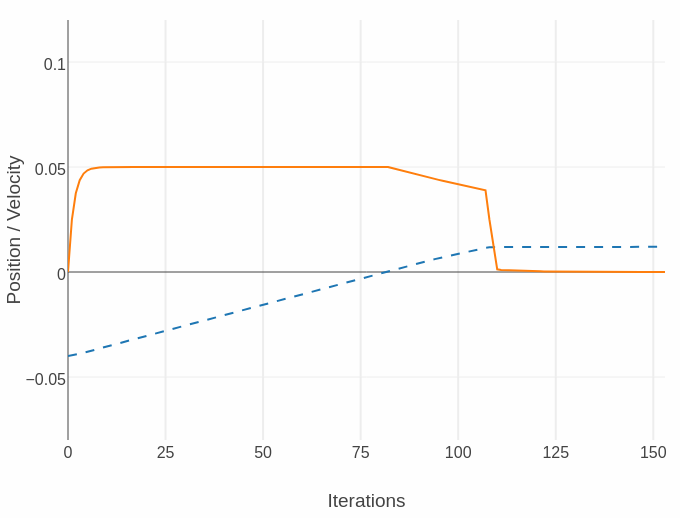
\includegraphics[width=0.49\linewidth]{controllers/basic_0.png}}
	\end{subfigure}
	\begin{subfigure}[][Joint $q_{1}$]
		{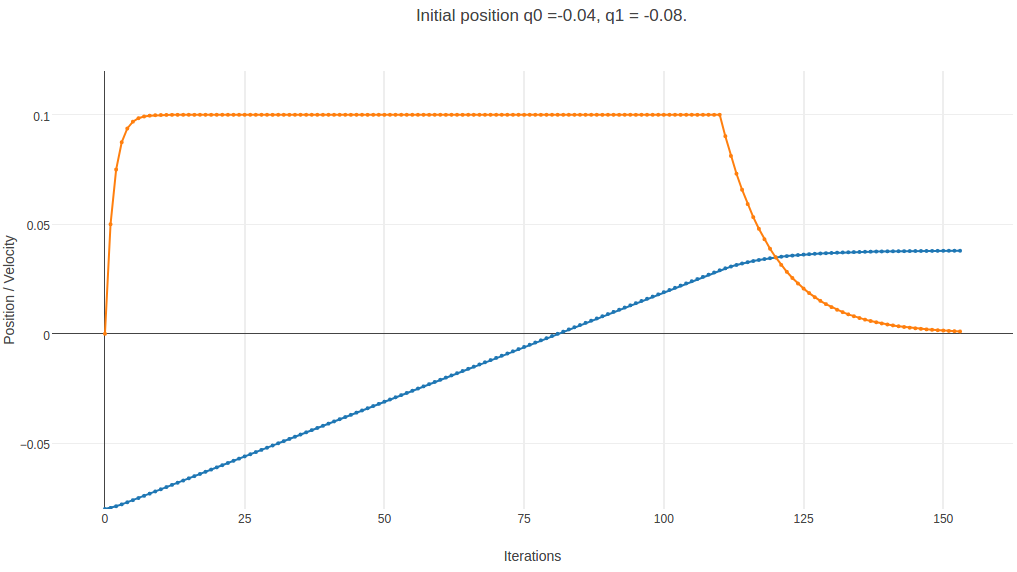
\includegraphics[width=0.49\linewidth]{controllers/basic_1.png}}
	\end{subfigure}
	\vspace{-12pt}
	\caption[Basic 2 DOF controller: Joints trajectories]{Joints trajectories (blue). Each joint has different velocity(orange) and acceleration constraints.}
	\vspace{-10pt}
	\label{fig:basic}
\end{figure}
It can be seen that the velocity decreases once the EEF is approaching the desired position, also the joints do not reach the maximum velocity in the first time step. This is due to the acceleration constraint given by equations \ref{eq:accel0} and \ref{eq:accel1}, the maximum acceleration is calculated on every iteration with:
\begin{equation}
a_{n,max\_lim}\ \ =\ \ \frac{\dot{q}_{n,max} - a_{n,max}}{\dot{q}_{n,max}} + a_{n,max}
\end{equation} 
\begin{equation}
a_{n,min\_lim}\ \ =\ \ \frac{\dot{q}_{n,max} - a_{n,max}}{\dot{q}_{n,max}} - a_{n,max}
\end{equation}

where $n$ is the joint number and $a_{n,max}$ a constant acceleration limit.

\subsection{Joints goal and EEF goal}
This example allows to specify a goal position for one of the joints as well as for the EEF. Figures \ref{fig:joint_eef} and \ref{fig:joint_0} show the behavior of the EEF and both joints while reaching the specified goals. Each joint has different velocity and acceleration constraints.

In this controller, the weight vector is defined as $\vec{\omega} = [ \omega_{1},\ \omega_{2},\ \omega_{3},\ \omega_{4} ]$. Where $\omega_{1}$ and $\omega_{2}$ are the joint weights, $\omega_{3}$ is the weight of the slack factor and $\omega_{4}$ is the weight of the joint goal. Equation \ref{eq:a_constr} is rewritten as:

$$
\left( \begin{array}{c}
error \\
-q_{0,max} - q_{0} \\
-q_{1,max} - q_{1} \\
a_{0,min\_lim} \\
a_{1,min\_lim} \\
joint\_error
\end{array}
\right)	\leq 
\left[ \begin{array}{cccc}
1 & 1 & 1 & 0 \\
1 & 0 & 0 & 0 \\
0 & 1 & 0 & 0 \\
1 & 0 & 0 & 0 \\
0 & 1 & 0 & 0 \\
1 & 0 & 0 & 1 \\
\end{array}
\right] *
\left( \begin{array}{c}
\dot{q}_{0} \\
\dot{q}_{1} \\
\epsilon \\
\epsilon_j \\
\end{array}
\right) 
\leq \left( \begin{array}{c}
error \\
q_{0,max} - q_{0} \\
q_{1,max} - q_{1} \\
a_{0,max\_lim} \\
a_{1,max\_lim} \\
joint\_error
\end{array}
\right)
$$

Where $\epsilon_j$ is the slack factor for the joint goal and $joint\_error$ is the current error of the joint $q_{0}$ to the joint goal, given by $joint\_error = q_{0,des}\ -\ q_{0}$

\begin{figure}[H]
	\centering
	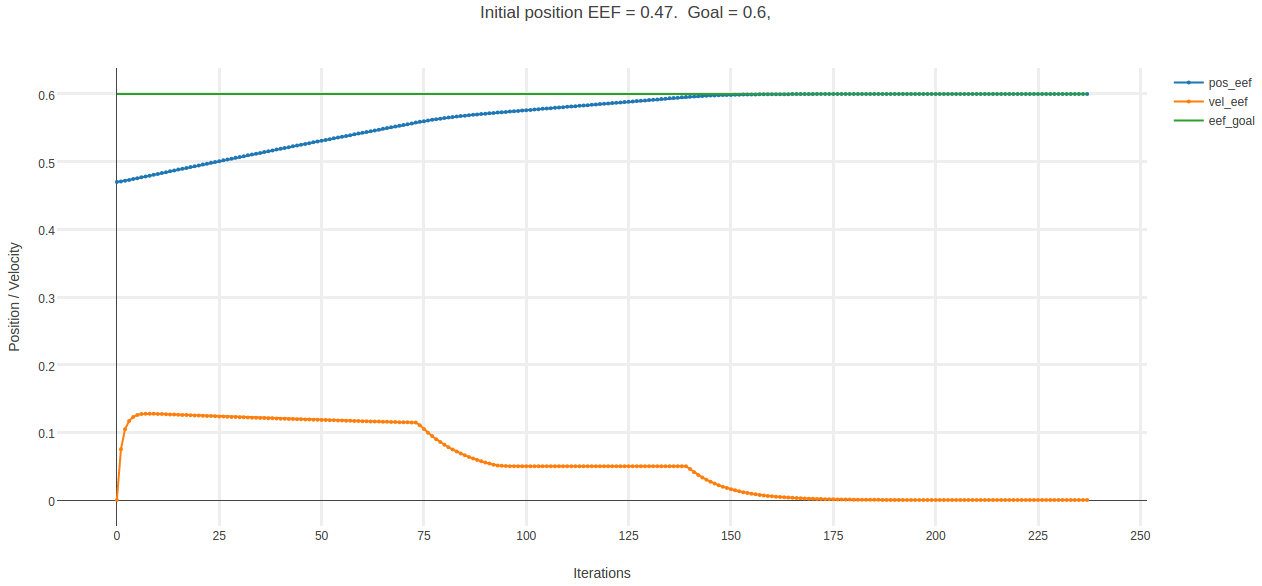
\includegraphics[width=0.9\linewidth, angle=0]{controllers/joint_eef.png}
	\vspace{-10pt}
	\caption[Joint and EEF goal: EEF trajectory]{Trajectory (blue), velocity (orange) and goal (green) of the EEF.}
	\vspace{-15pt}
	\label{fig:joint_eef}
\end{figure}
The initial position ot the EEF is $0.47$, and of the joints $q_{0}= 0.02$ and $q_{0}= -0.15$, respectively. Only a goal for the EEF and for the first joint, $EEF_{f}= 0.6$ and $q_{0f} = -0.25$. are specified.
\begin{figure}[H]
	\centering
	\begin{subfigure}[][Joint $q_{0}$]
		{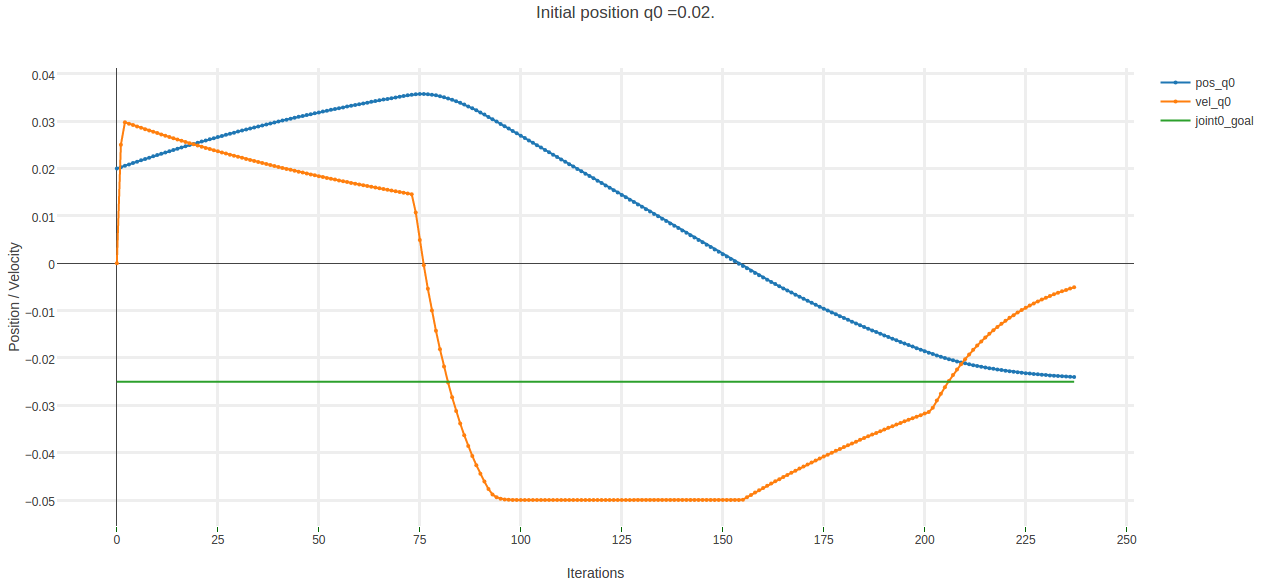
\includegraphics[width=0.49\linewidth]{controllers/joint_q0.png}}
	\end{subfigure}
	\begin{subfigure}[][Joint $q_{1}$]
		{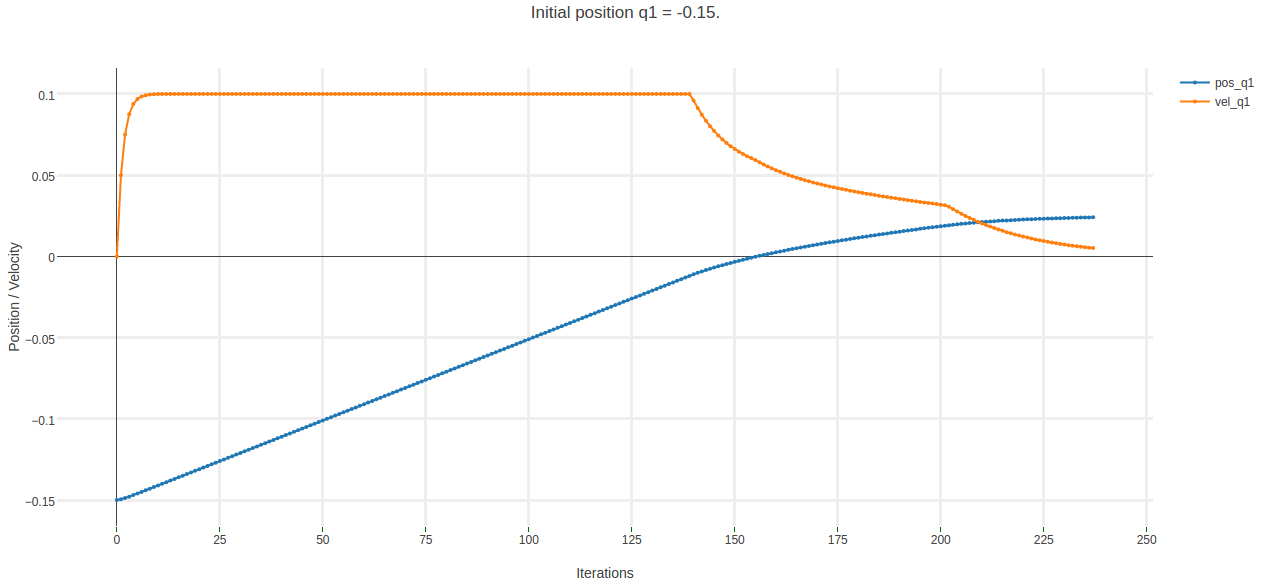
\includegraphics[width=0.49\linewidth]{controllers/joint_q1.png}}
	\end{subfigure}
	\vspace{-12pt}
	\caption[Joint and EEF goal: Joints Trajectories]{Trajectories (blue) and velocities (orange) of both joints and goal (green) of $q_{0}$.}
	\vspace{-10pt}
	\label{fig:joint_0}
\end{figure}

It can be seen in figure \ref{fig:joint_0} that one of the joints changes direction after around 75 iterations. This happens because the goal of the EEF and of the joint are in different directions, the system tries to minimize first the EEF error and afterwards the one of the joint. This behavior suggest  that it might be better to split the problem when goals for the joints are specified, where in the first part the joint goals are satisfied and kept constant and in the second part the EEF is reached.


\subsection{Position range as goal for the EEF}

In this example, the goal specified for the EEF is not one specific position, but a range, where any point in this area is a valid goal for the EEF.
\begin{figure}[H]
	\centering
	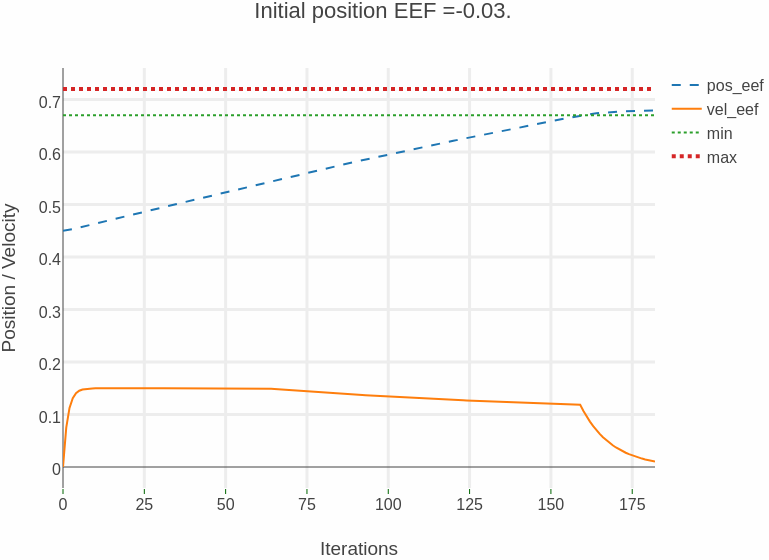
\includegraphics[width=0.9\linewidth, angle=0]{controllers/range_1.png}
	\vspace{-10pt}
	\caption[Position range as goal]{Trajectory (blue) and velocity (orange) of the $EEF$, the goal range is between the green and red lines.}
	\vspace{-15pt}
	\label{fig:range_1}
\end{figure}
Figure \ref{fig:range_1} shows the trajectory followed by the EEF while reaching the goal, it stops shortly after entering the given goal range. If a specific point inside this range is preferred as goal, an \textit{attractor} can be created,so that the EEF will try to reach the point defined by the attractor, but, if it is not possible, it will stay in the goal range.

To achieve this behavior, matrix $A$ and it's limits, $lbA$ and $ubA$, are modified, rewriting equation \ref{eq:a_constr} as:

$$
\left( \begin{array}{c}
error \\
-q_{0,max} - q_{0} \\
-q_{1,max} - q_{1} \\
a_{0,min\_lim} \\
a_{1,min\_lim} \\
range_{min} - q_{eef}
\end{array}
\right)	\leq 
\left[ \begin{array}{cccc}
1 & 1 & 1 & 0 \\
1 & 0 & 0 & 0 \\
0 & 1 & 0 & 0 \\
1 & 0 & 0 & 0 \\
0 & 1 & 0 & 0 \\
1 & 1 & 0 & 1 \\
\end{array}
\right] *
\left( \begin{array}{c}
\dot{q}_{0} \\
\dot{q}_{1} \\
\epsilon \\
\epsilon_r \\
\end{array}
\right) 
\leq \left( \begin{array}{c}
error \\
q_{0,max} - q_{0} \\
q_{1,max} - q_{1} \\
a_{0,max\_lim} \\
a_{1,max\_lim} \\
range_{max} - q_{eef}
\end{array}
\right)
$$

Where $\epsilon_r$ is the slack factor for the goal range, the error is calculated using the attractor (goal) $error = attr - q_{eef}$. Here, the weight vector is defined as $\vec{\omega} = [ \omega_{1},\ \omega_{2},\ \omega_{3},\ \omega_{4} ]$. Where $\omega_{1}$ and $\omega_{2}$ are the joint weights, $\omega_{3}$ is the weight of the attractor and $\omega_{4}$ is the weight of the goal range. The constraints of the state vector (eq. \ref{eq:state_constr}) is rewritten as:

$$
\left( \begin{array}{c}
-\dot{q}_{0,max} \\
-\dot{q}_{1,max} \\
-\epsilon_{max} \\
\epsilon_{r,max} \\
\end{array}
\right)	\leq 
\left[ \begin{array}{cccc}
\omega_{1} & 0 & 0 & 0 \\
0 & \omega_{2} & 0 & 0 \\
0 & 0 & \omega_{3} & 0 \\
0 & 0 & 0 & \omega_{4} \\
\end{array}
\right] *
\left( \begin{array}{c}
\dot{q}_{0} \\
\dot{q}_{1} \\
\epsilon \\
\epsilon_r \\
\end{array}
\right) 
\leq \left( \begin{array}{c}
\dot{q}_{0,max} \\
\dot{q}_{1,max} \\
\epsilon_{max} \\
\epsilon_{r,max} \\
\end{array}
\right)
$$
\\
Figures \ref{fig:range_eef} to \ref{fig:range_q1} show the behavior of the EEF and joints, in this example the attractor was set at $0.7$, with the range between $0.67$ and $0.72$. It can be seen how the EEF reaches the goal set by the attractor, instead of just staying at the range borders. 
\begin{figure}[H]
	\centering
	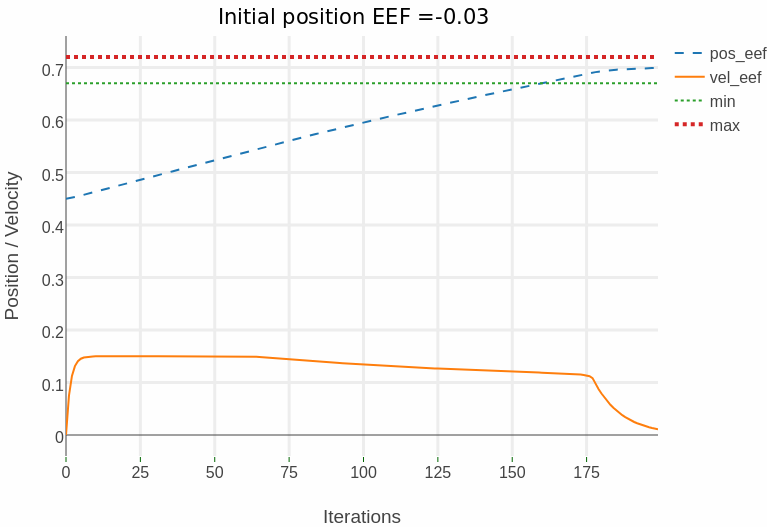
\includegraphics[width=0.8\linewidth, angle=0]{controllers/range_eef.png}
	\vspace{-10pt}
	\caption[Position range with attractor: EEF]{Trajectory (blue) and velocity (orange) of the EEF, here an attractor is defined inside the range.}
	\vspace{-15pt}
	\label{fig:range_eef}
\end{figure}
\begin{figure}[H]
	\centering
	\begin{subfigure}[][Joint $q_{0}$]
		{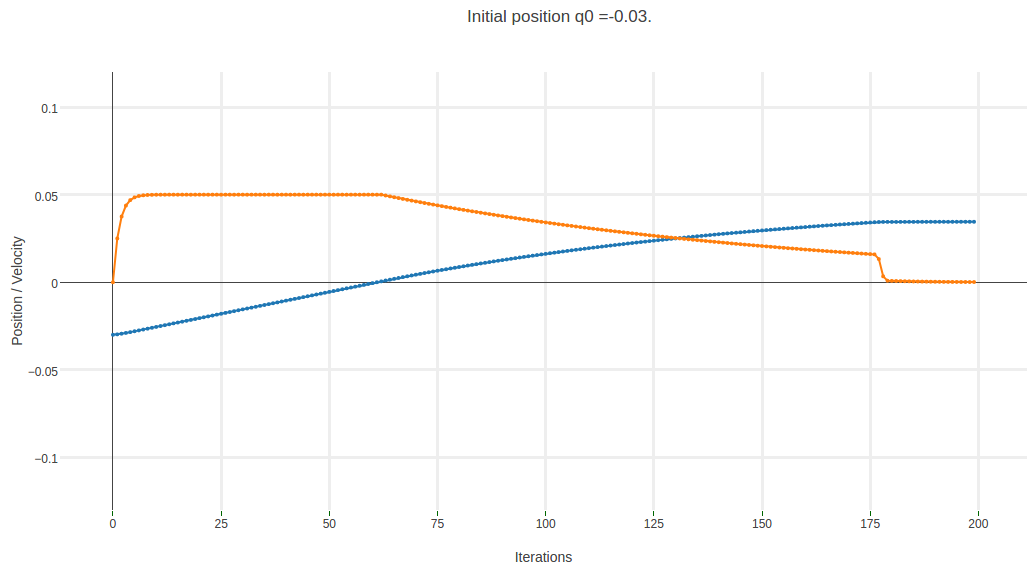
\includegraphics[width=0.49\linewidth]{controllers/range_q0.png}}
	\end{subfigure}
	\begin{subfigure}[][Joint $q_{1}$]
		{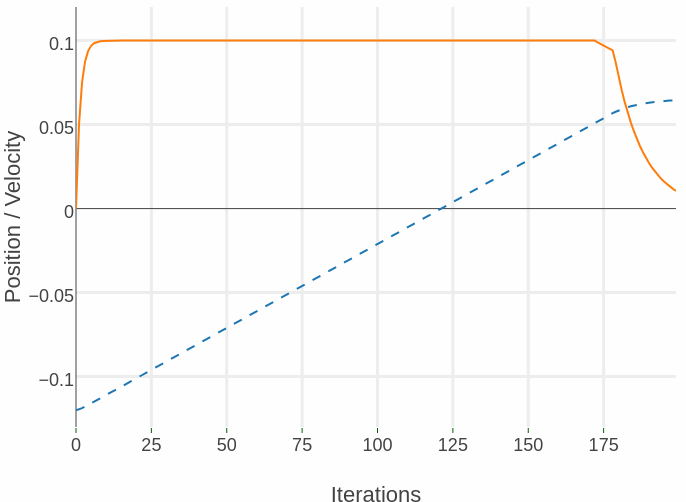
\includegraphics[width=0.49\linewidth]{controllers/range_q1.png}}
	\end{subfigure}
	\vspace{-12pt}
	\caption[Position range with attractor: Joints]{Trajectory (blue) and velocity (orange) of both joints}
	\vspace{-10pt}
	\label{fig:range_q1}
\end{figure}
The weight of the attractor is set higher than the range's weight, this means that the cost of reaching the point defined by the attractor is higher than just going inside the range. By doing this, the optimization algorithm prioritizes moving the EEF to the given range. Modifying these weights determine how close will the EEF come to the attractor.



...

....
....

....

\subsection{Multiple goals for the EEF}
\subsection{Dynamic weights}
\subsection{Trajectory parametrization}
\section{Trajectory evaluation}
\subsection{One-hand Grasping}
\subsection{Dual-hand Grasping}

\section{Hardware and Software requirements}
\label{subsec:software}

This project was developed in a computer running on Ubuntu 14.04, no special hardware is required to execute the generated code.

However, the user needs to have some programs and packages installed: 
\begin{itemize}
	\item \textbf{ROS:} With a configured workspace. The ROS distro used was \textit{indigo}
	\item \textbf{MoveIt!:} Requires previous installation of ROS
	\item \textbf{UR3 driver:} A recomended one is \texttt{ur\_modern\_driver}
	\item \textbf{Boxy repositories:} The \texttt{iai\_boxy} and \texttt{iai\_robots} from the IAI github repository\footnote{\url{https://github.com/code-iai}}
	\item \textbf{UR3 MoveIt configuration:} The code generated as a result of this project\footnote{\url{https://github.com/mgvargas/Moveit_config}}
\end{itemize}


After installing ROS and MoveIt!, the user has to download the specified repositories from Github. 

